

\section{Introduction}
\begin{figure}
\centering
{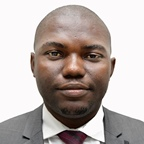
\includegraphics[width=5cm, height=7cm]{ogundeko.JPG}}
\end{figure}

My name is Abiola Ogundeko, a PhD student in Security Engineering, College of Engineering and Applied Science, University of Colorado, Colorado Springs, USA. My research thrust are using formal methods and Federated Learning approach in solving security related problems in Cyber-Physical Systems (CPS). I am a member of Embedded Systems Security Lab (ESSL) which is headed by my advisor, Acting Professor, Dr. Gedare Bloom. We are currently working on a project funded by National Science Foundation (NSF) awarded under the Office of Advance Cyberinfrastructure (OAC) with award number 123456. The project entails providing security in various forms for a scientific infastructure called Experimental Physics and Industrial Control Systems (EPICS). 
\subsection{Goals for CS6000 Class}
I am enthusiastic about CS6000 in a number of ways. First, Professor Terrance E. Boult is well-known in academia most especially in the Computer Science domain as an iconic scholar with impeccable records of achievement.Secondly, he is the visionary behind the Bachelor of Innovation as well as El Pomar Endowed Chair of Innovation and Security and Professor of Computer Science at the University of Colorado at Colorado Springs (UCCS). Without much ado, I have the following objectives to accomplish by the end of the class:
\begin{itemize}
    \item Get at least one survey paper published on or before the end of the class.
    \item Get some strategies, insights and tricks into getting publications in good venues.
    \item Understand the DO's and DONT's of research in Computer Science domain.
    \item Improve my research methodologies skills that will aid towards successful completion of my PhD program at UCCS.
    \item Establish a relationship with him to the point that I can get advise and research directions from his wealth of knowledge and experience.
\end{itemize}

\subsection{Proposed lessons to gain from CS6000 Class.}
Having realized CS6000 class is going to be taken online during the Spring 2020 semester due the COVID-19 pandemic, I was unhappy about it.However, since the commencement of the class I have been impressed by the way it is being conducted. The interactive discussions going on Canvass portal, the uploaded YouTube videos, and the weekly Journal writing task that we are saddled with. I feel elated and hope to gain the following knowledge at the end of the course:
\begin{enumerate}
    \item Improve my writing skills up to required level of getting papers published.
    \item Improve my paper reading skills by adopting the five steps of reading papers.
    \item How to effectively conduct experiment in Computer Science domain. 
    \item How to review papers effectively and efficiently.
    \item Lastly, spur me to start working on my thesis towards successful defense and graduation.
\end{enumerate}

\subsection{Personal profile}
I am the penultimate child in a family of 5 children. I started my PhD program at Howard University and got transferred to UCCS as a result of my professor quest to join him at UCCS. I am married and blessed with 3 kids although they are still  in Nigeria. I hope to bring them soon. Aside that, I have been enjoying every bit of my PhD journey and I hope to complete it with flying colors. I love Colorado as a state with beautiful weather and mountainous views. There are lots of scenery places to visit in Colorado.



\section{Assignment tasks in the Video}
The first exercise asked us to search for twenty-five papers related to our research interest. I used Google scholar with two search iterations. First, I searched with the title: Federated Learning and got a number of outputs which I selected from. My selection was based on a number of criteria such as the number of citations, published versus archive, how recent was the paper, and so on. Thereafter, because I realized I am interested in a survey paper of existing work on Federated Learning (FL), I further searched with the string "Federated Learning: A survey" and a number of survey related papers were taking considering aforementioned criteria. I noticed a number of this papers are archived papers and few published ones have few citations that spurred my interest to snowballed into citations in a forward and backward manner to get more than twenty-five (25) papers. 
The second exercise entails using Google Scholar to find a good paper written by my advisor. I searched with the string "Gedare Bloom" and further clicked on his name up as shown in Fig 1. I selected the paper titled " Design patterns for the industrial internet of things"  based on the venue, number of citations (48), first authorship and lastly the fact that I have read the paper, year the paper was published ie. 2018 still very recent\cite{b2}. 
Furthermore, the sub task in the second exercise entails finding all papers written by Professor Terrance Boult published in IEEE Transactions on Pattern Analysis & Machine Intelligence in the last five years. I made use of advance search option on Google Scholar with search string "author:Terrance author:Boult source:IEEE source:Transactions source:on source:Pattern source:Analysis source:and source:Machine source:Intelligence" with customs range setting of the year 2015 - 2019 as shown in Fig 2. The paper titled: The extreme value machine \cite{b1}.





\section{Survey on Federated Learning}
As stated earlier in Section 1, one of our research trust is the use of Federated Learning (FL) to solve security related problem in Cyber-Physical systems. Having reviewed existing literature, I realized that Qiang et al\cite{b3} elaborate on the concepts and applications of Federated learning by describing different architectures that exist such as Horizontal, Vertical and Federated Transfer learning. Also is the work of Mohammed Aledhari et al that looked out various Machine Learning (ML) algorithms, framework, open source systems and applications used in FL\cite{b7}. However, despite other survey papers in FL \cite{b17, b14, b16, b8,b9,b11}, to the best of our knowlede, we are the first to look at reviewing existing literature's with respect to conducting a survey for the use of Federated Learning in Industrial Control Systems. Our future work is the use of FL algorithm to solve security challenges in ICS by training and testing a myriads of ICS dataset that exist our there.



